\section{Qu’est-ce ce qu’un property graph}
\subsection{Définition}

Les graphes de propriétés (Property graphs) permettent d'associer facilement des propriétés (paires clé-valeur) aux sommets et aux arêtes des graphes, et ils permettent des opérations d'analyse basées sur des relations entre un grand nombre de données.\\
Au contraire aux graphes classiques, dont les élèves dans les universités sont habituées où tous les sommets/arrêtes sont du même type (sommets des villes, arrêtes des coûts) le Property graphe est composé des plusieurs types comme le cas d’une base de données relationnel où on trouve différentes types de tables (Table personne, table transaction).\\
La carte conceptuelle ci-dessous explique les principaux aspects utilisés dans le contexte des graphes avec propriétés (Property graphs).\\

\begin{figure}[h!]  
  \centering
    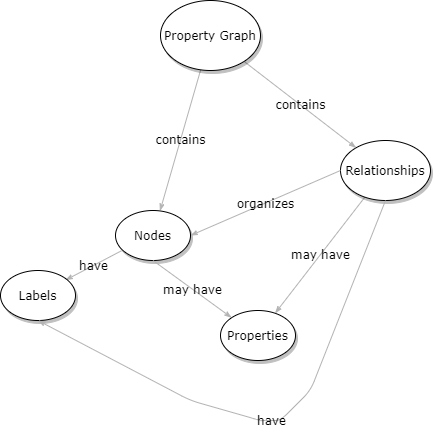
\includegraphics[width=0.8\textwidth]{chapitre2/Figures/PropertyGraph.png}
  \caption{Carte conceptuelle d'un property graph}
\end{figure}

\newpage
\textbf{Example :}
\begin{figure}[h!]  
  \centering
    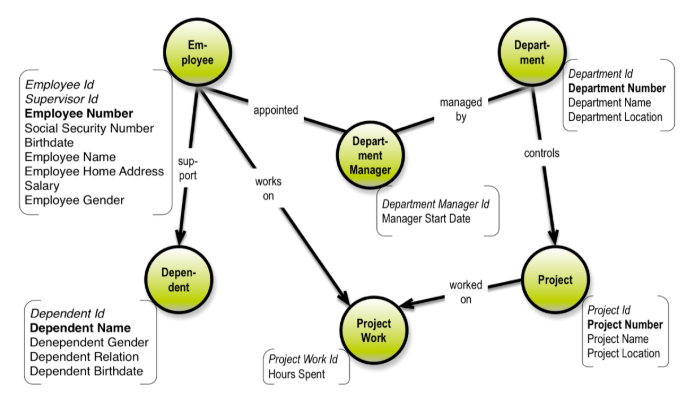
\includegraphics[width=1\textwidth]{chapitre2/Figures/PropertyGraphExample.PNG}
  \caption{Exemple d'un property graph}
\end{figure}

Dans cet exemple, nous pouvons observer ce qui suit:

\begin{itemize}[label=\textbullet]
\item  Chaque nœud (en vert) a une relation orientée (arêtes) avec un autre nœud.
\item  Chaque nœud/arrête a une étiquette (par exemple, le nœud avec l'étiquette Employee est lié à un nœud étiqueté Dependent avec une arête étiquetée support).
\item  Chaque type de nœud a son propre ensemble de propriétés. Par exemple le nœud Department à comme propriétés ; {Department Id, Department Number, Department  Name, Department Location}.
\item  Les arêtes n'ont pas de propriétés.
\end{itemize}

\subsection{Le property graphe dans PGX}
En PGX en distingue entre deux types des graphes selon les propriétés de ses composant (sommets et arrêtes):

\begin{itemize}[label=\textbullet]
\item  \textbf{Les graphes homogènes :}
Un graphe est dit homogène si tous ces sommets/arrêtes ont les mêmes propriétés, mais pas nécessairement que les sommets ont les mêmes propriétés que les arrêtes. C’est plus ou moins le cas des graphes qu’on introduit dans les cours magistraux des universités mais dans ces cours tous les sommets et arrêtes sont du même type (ex. les villes et les routes qui les relies). Ici les types des sommets/arrêtes peuvent être différentes comme dans la figure 11, ou on a des sommets de type Employee, Project …etc. La graphe dans la figure 11 pour qu’il soit homogène, il doit avoir dans ces sommets/arrêtes les mêmes propriétés, par exemple, les sommets de type Project devront comporter une propriété « Birthdate » comme chez les sommets de type Employee.
\item  \textbf{Les graphes hétérogènes :}
Les graphes hétérogènes sont comme les graphes homogènes sauf que chaque sommets/arrêtes à ces propres propriétés comme montre la figure 11.
\end{itemize}

Actuellement PGX.SM support des graphes hétérogènes tandis que PGX.D, support des graphes homogènes. Ceci est dû au fait que PGX.D est plus récent par-rapport à PGX.SM.\\
Les graphes homogènes bien que plus simples à implémenter, ils introduisent des coûts non désirables, comme la consommation des plus de mémoire, et les temps de chargement en mémoire car il y a plus des propriétés que ceux nécessaires.\\
\newpage
Dans PGX un Property graph est représenté par un fichier JSON qui décrit en détail comment les données du graphe sont structures et comment il sera chargé en mémoire.\\

\begin{figure}[H]  
  \centering
    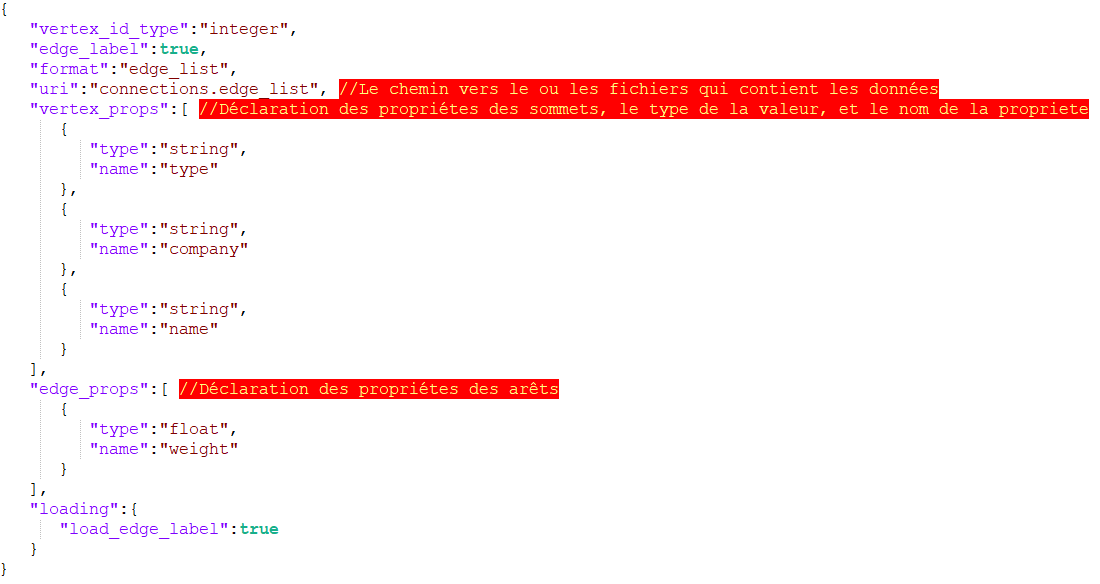
\includegraphics[width=1.15\textwidth]{chapitre2/Figures/GraphJSON.PNG}
  \caption{Exemple d'un fichier JSON que contient des métadonnées d'un graphe}
\end{figure}